
\abstract*{
XcalableMP(XMP) supports a global-view model that allows programmers to define global data and to map them to a set of processors, which execute the distributed global data as a single thread. In XMP, the concept of a coarray is also employed for local-view programming.
 In this study, we port Gyrokinetic Toroidal Code - Princeton (GTC-P), which is a three-dimensional gyrokinetic PIC code developed at Princeton University to study the microturbulence phenomenon in magnetically confined fusion plasmas, to XMP as an example of hybrid memory model coding with the global-view and local-view programming models.
 In local-view programming, the coarray notation is simple and intuitive compared with Message Passing Interface (MPI) programming while the performance is comparable to that of the MPI version. Thus, because the global-view programming model is suitable for expressing the data parallelism for a field of grid space data, we implement a hybrid-view version using a global-view programming model to compute the field and a local-view programming model to compute the movement of particles. The performance is degraded by 20\% compared with the original MPI version, but the hybrid-view version facilitates more natural data expression for static grid space data (in the global-view model) and dynamic particle data (in the local-view model), and it also increases the readability of the code for higher productivity.
}

\abstract{
XcalableMP(XMP) supports a global-view model that allows programmers to define global data and to map them to a set of processors, which execute the distributed global data as a single thread. In XMP, the concept of a coarray is also employed for local-view programming.
 In this study, we port Gyrokinetic Toroidal Code - Princeton (GTC-P), which is a three-dimensional gyrokinetic PIC code developed at Princeton University to study the microturbulence phenomenon in magnetically confined fusion plasmas, to XMP as an example of hybrid memory model coding with the global-view and local-view programming models.
 In local-view programming, the coarray notation is simple and intuitive compared with Message Passing Interface (MPI) programming while the performance is comparable to that of the MPI version. Thus, because the global-view programming model is suitable for expressing the data parallelism for a field of grid space data, we implement a hybrid-view version using a global-view programming model to compute the field and a local-view programming model to compute the movement of particles. The performance is degraded by 20\% compared with the original MPI version, but the hybrid-view version facilitates more natural data expression for static grid space data (in the global-view model) and dynamic particle data (in the local-view model), and it also increases the readability of the code for higher productivity.
}

%1
\section{Introduction\label{sec1}}

In XMP, the global-view model allows programmers to define global arrays, which are distributed to processors by adding the directives. Some typical communication patterns are supported by directives, such as data exchange between neighbor processors in stencil computations.
In contrast to the global-view model, the local-view model describes remote memory access using the node (processor) index. This operation is implemented as one-sided communication. XMP employs the coarray concept from Coarray Fortran as a local-view programming model. A coarray is a distributed data object, which is indexed by the coarray dimension that maps indices to processors.
In XMP, the coarray is defined in C as well as Fortran. In the local-view model, a thread on each processor executes its own local computations independently with remote memory access to data located in different processors by coarray access. The local-view model requires that programmers define their algorithms by explicitly decomposing the data structures and controlling the flow in each processor. The data view is similar to that in MPI, but coarray remote access provides a more intuitive view of accessing the data in different processors, thereby increasing productivity.

In this chapter\footnote{
  The original version of this chapter was published in: 
  Keisuke Tsugane, Taisuke Boku, Hitoshi Murai, Mitsuhisa Sato, William M. Tang, Bei Wang, ``Hybrid-view programming of nuclear fusion simulation code in the PGAS parallel programming language XcalableMP.'' Parallel Computing 57: 37-51 (2016).
  }, we consider a hybrid-view programming approach, which combines the global-view and local-view models in XMP according to the characteristics of the distributed data structure of the target application.
The global-view model allows programmers to express regular parallel computations such as domain decomposition with stencil computation in a highly intuitive manner simply by adding directives to a serial version of code. However, it is difficult to describe parallel programs in the global-view model when more irregular communication patterns and complex load balancing are required on the processing. Thus, local-view programming is necessary in these situations.

We apply this hybrid-view programming for Gyrokinetic Toroidal Code - Princeton (GTC-P)\cite{GTC-P1}, which is a large-scale plasma turbulence code that can be applied at the International Thermonuclear Experimental Reactor (ITER \cite{ITER}) scale and beyond for next-generation nuclear fusion simulation.
The GTC-P is an improved version of the original GTC\cite{GTC} and it is a type of gyrokinetic Particle-in-Cell (PIC) code with two basic data arrays: global grid data that corresponds to the physical problem space and particle data that corresponds to particles moving around the grid space. The original GTC-P was written in C as a form of hybrid programming with OpenMP and MPI. In this code, the grid data and particle data are mapped onto MPI processes and exchanged. As found with most codes of this type, it is difficult to manage complex data distributions and communication for both grid data and particle data during code development. Furthermore, to simulate the microturbulence phenomenon in plasmas for magnetically confined fusion devices, non-flat domain decomposition is necessary in one dimension, as well as parallelizing multiple dimensions, to obtain accurate large-scale simulations. Therefore, the number of computations becomes extremely large for next-generation and large-scale reactors such as ITER.

We consider both types of data models in XMP, i.e., global-view and local-view models, which are suitable for representing grid space data and particle data, respectively, because of their data distribution and communication pattern. In this study, we implement the GTC-P code in two ways: using XMP with a local-view only model, and with a combination of local-view and global-view models, where we evaluate the performance and productivity of these approaches. As the preliminary result, we implemented and evaluated the GTC-P in XMP hybrid-view model\cite{HYBRID}. Moreover, we indicate the causes of performance degradation for GTC-P in XMP and evaluate the GTC-P of hybrid versions written in XMP+OpenMP and MPI+OpenMP in this study.

The remainder of this chapter is organized as follows.
Next, we briefly describe the GTC-P nuclear fusion simulation code in Section \ref{sec2}. Section \ref{sec3} describes the implementation of GTC-P using
Hybrid programing model of XMP. We report the performance and productivity evaluation in Section \ref{sec4}, and related works in Section \ref{sec5}. Finally, we conclude our study in Section \ref{sec6}.

%3.3

%4
\section{Nuclear Fusion Simulation Code\label{sec2}}
Typical methods used to simulate the microturbulence phenomenon in magnetically confined fusion plasmas include the Monte Carlo method and the PIC method. In this study, we only consider the gyrokinetic PIC method among them as a target application to explain the GTC and GTC-P code briefly.

\begin{figure}[t]
\begin{center}
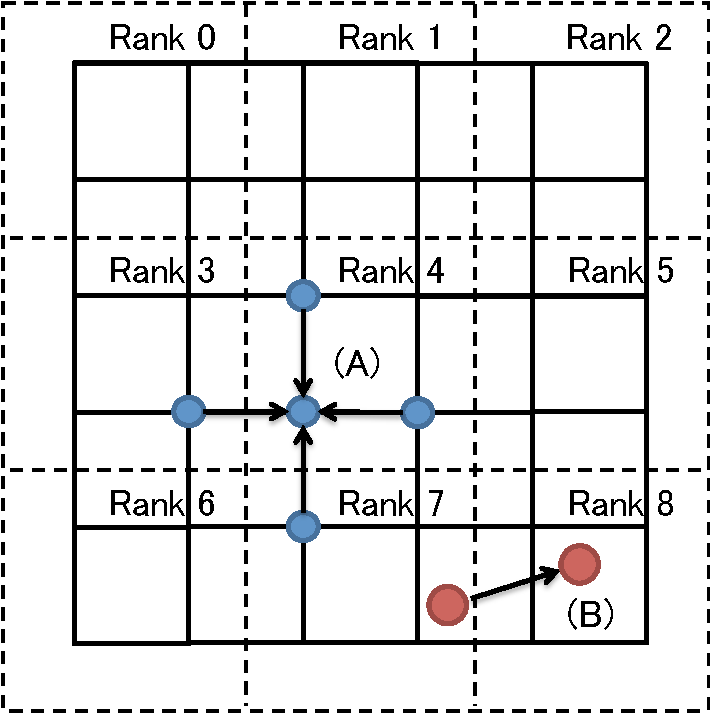
\includegraphics[width=5.5cm,bb=0 0 341 342]{./figure/picfig.pdf}
\caption{Image from a gyrokinetic PIC simulation with a two-dimensional block distribution; (A) Calculation of the field using the nearby grid points, and (B) the movement of a particle. The dashed lines indicate processor boundaries. }
\label{picfig}
\end{center}
\end{figure}


\begin{figure}[t]
\begin{center}
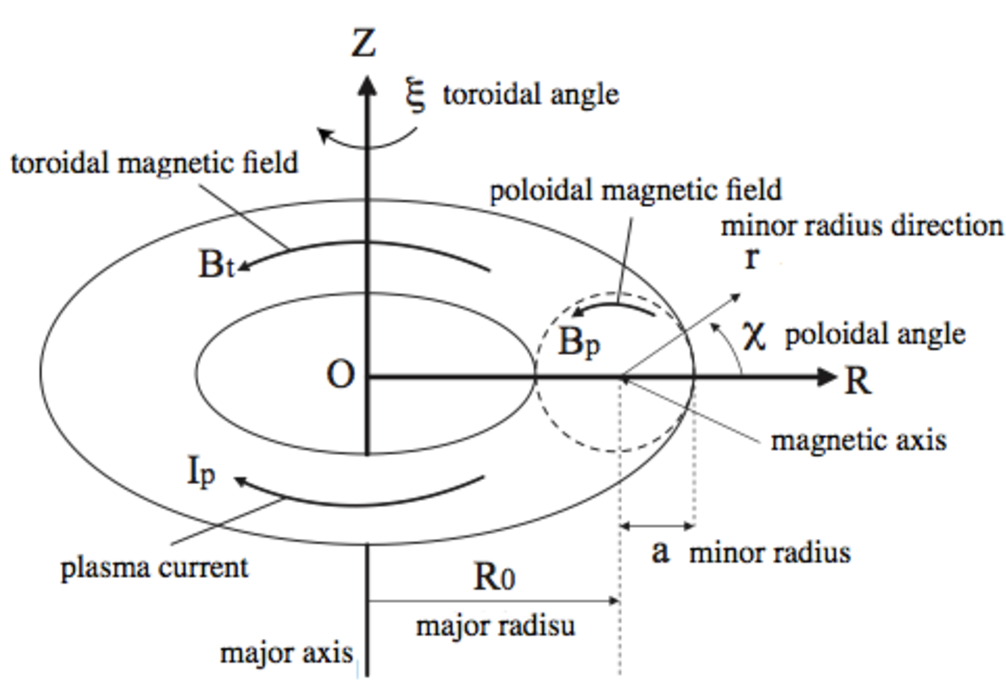
\includegraphics[width=7.7cm,bb=0 0 482 334]{./figure/torus.pdf}
\caption{Conceptual image of the three-dimensional torus space in GTC-P\cite{NUGA}.}
\label{torus}
\end{center}
\end{figure}

%4.1
\subsection{Gyrokinetic PIC Simulation}
The simulation of the gyrokinetic PIC method uses a space grid to calculate the field and for the particle trajectory calculation, which does not depend on the grid when moving in the free space. Figure \ref{picfig} shows an image of a gyrokinetic PIC simulation with a two-dimensional block distribution. The typical behavior of the gyrokinetic PIC code is as follows.

\begin{enumerate}
\item Add the charge of the particle to the nearby grid points.
\item Solve the electric field affected by the electrostatic potential by calculating the charge density of the nearby grid points using Poisson's equation.
\item Interpolate the electric field in the current position based on each particle in the nearby grid points and move the position of the particle in the space.
\end{enumerate}

During each step, a process must communicate with another if that process holds the data for the space in the grid that is affected, as shown in Figure \ref{picfig} (A), or if the particle data move from or to that process, as shown in Figure \ref{picfig} (B). Based on the above, if the size of the distributed domain, e.g., the grid in Figure \ref{picfig}, is not changed, the data distribution employed in the global-view programming model is suitable and the communication between nearby grid points can be described by the {\tt reflect} directive in XMP coding.
In contrast, if the number of particles on each distributed domain changes dynamically during each time step of the simulation, such as particle motion, coarray communication is required using local-view programming.

\begin{figure}[t]
\begin{center}
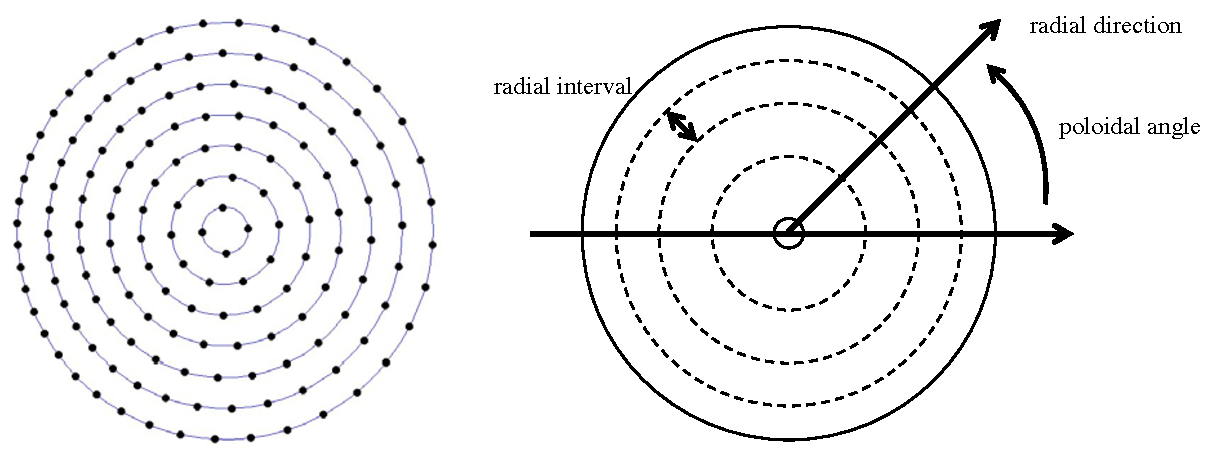
\includegraphics[width=10cm,bb=0 0 585 218]{./figure/poloidal.pdf}
\caption{Example showing the grid points on the poloidal plane in GTC-P\cite{POLOIDAL} (left). Image of the radial domain decomposition on poloidal plain. The dashed line shows the border of the decomposition (right).}
\label{poloidal}
\end{center}
\end{figure}


\begin{figure}[t]
\centering
{\scriptsize
\begin{minipage}{11cm}
\begin{lstlisting}
double f[X][Y]; /* Electric field data */
double p[N]; /* Particle data */
double send[N], recv[N]:[*];
#pragma xmp align f[i][j] with T(i, j)
#pragma xmp shadow f[1:1][1:1]

for(t=0; t<TIME; t++) {
  /* Calculate the grid-related work */
  #pragma xmp reflect(f)
  /* Calculate the particle-related work */
  /* Pack the communication elements from array "p" to array "send" */
  /* Calculate the destination process "pe" and communication size "icount" */
  recv[0:icount]:[pe] = send[0:icount];
  xmp_sync_all(NULL); /* Synchronization */
}
\end{lstlisting}
\end{minipage}
}
\caption{Example showing the implementation of a gyrokinetic PIC simulation with XMP.}
\label{picxmp}
\end{figure}


%4.2
\subsection{GTC}
GTC is a three-dimensional (3D) gyrokinetic PIC code, which was developed by DOE SciDAC, UC Irvine, etc.\cite{GTC} for studying the microturbulence phenomenon in plasmas for magnetically confined fusion devices. Figure \ref{torus} shows a conceptual image of a 3D torus physical space. GTC treats the physical space and the movement of particles in three directions: the toroidal direction around the major axis, the poloidal direction around the magnetic axis, and the radial direction of the minor radius from the magnetic axis. The cross-section of the toroidal direction is known as the poloidal plane. GTC-P is a modified version of GTC, where there are several differences in the parallelization scheme. Moreover, GTC-P is implemented as two versions in the C and Fortran languages, whereas the original GTC is coded in Fortran. In this study, we focus on the C implementation of GTC-P.

GTC parallelizes the problem according to three levels. Processing on the space grid domain in the toroidal direction and the processing of particles in each domain are mapped onto MPI processes. Also, the grid-related calculation and particles in each distributed domain are further subdivided using OpenMP for each process. GTC-P has four levels of parallelism with additional parallelism in the radial direction. The total number of MPI processes that need to be executed is $N_t \times N_r \times N_{rp}$, where $N_t$ is the number of domains decomposed in the toroidal direction, $N_r$ is the number of domains decomposed in the radial direction, and $N_{rp}$ is the number of particles decomposed in each of the distributed domains.

There is a difference in the number of grid points on the poloidal plane, as demonstrated in Figure \ref{poloidal} (left). The toroidal domain can be distributed with equally sized intervals, but the radial domain cannot be distributed with equally sized intervals due to the large difference in the domain size depending on its position in space. Therefore, in order to align as much as possible the number of grid points to be mapped on each process, the outer area of the radial domain is distributed as short radial interval and its inner area is distributed as long radial interval, such as Figure \ref{poloidal} (right).

GTC-P has mainly six computational kernels. The {\tt charge} kernel deposits the charge from particles onto the grid using the 4-point approximation of nearby grid points. The {\tt poisson}, {\tt field}, and {\tt smooth} kernels solve the gyrokinetic Poisson's equation, compute an electric field, and smooths the charge and potential with a filter on the grid, respectively. The {\tt push} kernel interpolates the electric field onto particles using the field. The {\tt charge} and {\tt push} kernels account for large percentage of the elapsed time in this simulation \cite{GTC-P1}\cite{GTC-P2}.

\begin{figure}[t]
\centering
{\scriptsize
\begin{minipage}{11cm}
\begin{lstlisting}
/* send # of particles to right neighbor and recv from left neighbor */
MPI_Sendrecv(&nsendright, 1, MPI_INT, right_pe, sendtag,
               &nrecvleft, 1, MPI_INT, left_pe, recvtag, comm, &status);
/* send particles to right neighbor and recv from left neighbor */
MPI_Sendrecv(sendright, nsendright, MPI_DOUBLE, right_pe, sendtag, 
               recvleft, nrecvleft, MPI_DOUBLE, left_pe, recvtag, comm, status);
\end{lstlisting}
\end{minipage}
}
\caption{Particle data movement using MPI point-to-point communication in GTC-P}
\label{pmove_mpi}

\bigskip

\centering
{\scriptsize
\begin{minipage}{11cm}
\begin{lstlisting}
/* send # of particles to right neighbor */
nrecvleft:[right_pe] = nsendright;
/* send particles to right neighbor */
recvleft[0:nsendright]:[right_pe] = sendright[0:nsendright];
/* synchronization */
xmp_sync_image(right_pe, NULL);
\end{lstlisting}
\end{minipage}
}
\caption{Particle data movement using the coarray notation in GTC-P\label{pmove_xmp}}
\end{figure}

\begin{figure}[t]
\centering
{\scriptsize
\begin{minipage}{8.0cm}
\begin{lstlisting}
double *sendr, *recvl;

for(i=0;i<nloc_over;i++)
 sendr[i]=phitmp[i*(mzeta+1)+mzeta];

MPI_Sendrecv(sendr,nloc_over,MPI_DOUBLE,right_pe, 
     isendtag,recvl,nloc_over,MPI_DOUBLE,left_pe, 
     irecvtag,toroidal_comm,&istatus);
\end{lstlisting}
\end{minipage}
}
\caption{Exchange of grid points using MPI point-to-point communication in GTC-P.\label{mpi}}

\bigskip

\centering
{\scriptsize
\begin{minipage}{8.0cm}
\begin{lstlisting}
double Xsendr[nloc_over],Xrecvl[nloc_over]:[*];

for(i=0;i<nloc_over;i++)
 Xsendr[i]=phitmp[i*(mzeta+1)+mzeta];

Xrecvl[0:nloc_over]:[right_pe]=Xsendr[0:nloc_over];
xmp_sync_image(right_pe, NULL);
\end{lstlisting}
\end{minipage}
}
\caption{Exchange of grid points using the coarray notation in GTC-P.\label{coarray}}

\bigskip

\centering
{\scriptsize
\begin{minipage}{8.0cm}
\begin{lstlisting}
#pragma xmp reflect (phitmp) width (0,/periodic/1:0)
\end{lstlisting}
\end{minipage}
}
\caption{Exchange of grid points using the {\tt reflect} directive in GTC-P.\label{reflect}}
\end{figure}

%5
\section{Implementation of GTC-P by Hybrid-view Programming\label{sec3}}

In this section, we describe how to implement GTC-P using hybrid programming
model of XMP.

\subsection{Hybrid-view Programming Model}
XMP allows the use of hybrid-view programming, which combines the global-view and local-view models. The global-view model allows programmers to express regular parallel computations, such as domain decomposition with stencil computation, in a highly intuitive manner simply by adding directives to a serial version of the code. On the other hand, when the data distribution cannot be simply described in domain decomposition manner or the communication pattern is complicated, the global-view model is not suitable, and more dynamism is required to express the code naturally. Thus, the coarray notation provided by the local-view model is required in this case, and it is possible to program in a flexible manner using these models. 

Figure \ref{picxmp} shows a skeleton code of the implementation of a gyrokinetic PIC simulation with XMP. In this example, the grid uses a two-dimensional block distribution and each block has a sleeve area, which is used to calculate the field with the nearby grid points based on the {\tt shadow} directive. The particle movement is represented by the coarray notation where the communication elements are packed in the array {\tt send}. Based on the above, we describe the two implementations of GTC-P using XMP. First, we implement the XMP-localview version using coarray communication, which is equivalent to using MPI point-to-point communication with the exception of MPI collective communication (as shown below). Next, the XMP-hybridview version is implemented by describing the fields using a distributed array with the {\tt reflect} directive for overlapped sleeve area communication and the distributed data in the global-view programming model, as well as using the coarray notation to move the particle data. In addition, we use the {\tt bcast} and {\tt reduction} directives instead of MPI collective communication ({\tt MPI\_Bcast} and {\tt MPI\_Allreduce}) in both versions.

%5.1
\subsection{Implementation Based on the XMP Local-view Model: XMP-localview}
In GTC-P, the communication processes required to move particles between grids and to exchange grid points are represented by {\tt MPI\_Sendrecv} or {\tt MPI\_Isend/Irecv}, where most of the communication is performed between adjacent processes in one dimension. GTC-P has the steady state exchange of particles between neighboring subdomains. Because the number of particles changes dynamically, this implementation uses the coarray notation in the local-view programming model. 

Figures \ref{pmove_mpi} and \ref{pmove_xmp} show the particle data movement using MPI and the corresponding the coarray notation in GTC-P, respectively. In the exchange of coarray notation for particle data movement, it communicates the number of particles and the particle data, i.e., {\tt nsendright} and {\tt sendright}, with the adjacent process on the neighbor to the right. In addition, Figures \ref{mpi} and \ref{coarray} show the exchange of grid points using MPI and the corresponding coarray notation in GTC-P, respectively. In the example of the coarray notation for the exchange of grid points, after copying a value to a one-dimensional array, i.e., {\tt sendr} or {\tt Xsendr}, it communicates with the adjacent process on the neighbor to the right. Because the coarray notation is non-blocking communication, {\tt xmp\_sync\_image} on the sixth line of Figure \ref{pmove_xmp} and the seventh line of Figure \ref{coarray} are required to guarantee that communication has been completed between two processes, in this case, the neighboring ({\tt right\_pe}) and current processes.


\begin{figure}[t]
\centering
{\scriptsize
\begin{minipage}{8.0cm}
\begin{lstlisting}
#define n_t              2
/* Number of the toroidal domain decomposition */
#define n_r               4
/* Number of the radial domain decomposition. */
#define n_rp          2
/* Number of the particle decomposition. */

#define nloc_over          107722

double phitmp[nloc_over_all][2*n_t];
int  b[n_r*n_rp] 
 = {10967,10967,14086,14086,16164,16164,12644,12644};
/* Block size of each process in the "gblock" distribution. */

#pragma xmp nodes P2(n_r * n_rp, n_t)
/* Number of processes (nodes). */
#pragma xmp template T(0:nloc_over-1, 0:2*n_t-1)
/* Template length. */
#pragma xmp distribute T(gblock(b), block) onto P2
/*  Distribution format of the template. */
#pragma xmp align phitmp[i][j]    with T(i, j)
/* Alignment of an array with a template.*/
#pragma xmp shadow phitmp[0][1:0]
/* Assignment of the sleeve area. */
/* ... */
#pragma xmp loop (i, j) on T(i, j)
#pragma omp parallel for
  for (i = 0; i < nloc_over; i++)
    for (j = 0; j < mzeta; j++)
      phitmp[i][j] = func(i, j);
\end{lstlisting}
\end{minipage}
}
\caption{Example showing GTC-P implementation using the XMP global-view programming model.\label{gblock}}
\end{figure}


%5.2
\subsection{Implementation Based on the XMP Hybrid-view Model: XMP-hybridview}
In the XMP-hybridview implementation, all of the space grid data are denoted by a global-view model with compile-time mapping and the sleeve data are exchanged by XMP directives, whereas the particle data movements are denoted by a local-view model with the coarray notation, as shown Figure \ref{pmove_xmp}.
It is necessary to represent an unequal block size for domain decomposition in the radial dimension. Because this dimension's space grid is denoted in the global-view model, we apply the {\tt gblock} notation to represent it correctly in the same manner as the original MPI implementation. The {\tt gblock} notation can control the variable block size of each domain on the mapped space position. This feature is especially important for porting GTC-P onto XMP with a global-view model. Figure \ref{gblock} shows an example of the GTC-P implementation with the XMP global-view programming model using {\tt gblock}. The 11th line of this example denotes the block size distribution in the radial dimension. Because of describing the data distribution by global-view model, we can describe the loop distribution only to insert \texttt{loop} directive onto the serial code that is from the 28th to 30th lines of this example. In addition, OpenMP directives can be combined with XMP such as the 27th line.

The calculation of the grid-related works, such as the deposit of the charge from particles onto the grid using a 4-point approximation of grid points, the computation an electronic field, and the interpolation of the electronic field onto particles, are similar to 4-point stencil calculation on the poloidal plain. In these codes, we can describe the loop parallelization by inserting {\tt loop} directive onto the serial version. Appropriate directives are used for each dimension of the distributed array in XMP, and we further synchronize the sleeve data that overlap at each end of the distributed domain, which we can describe simply using the {\tt reflect} directive. Figure \ref{reflect} shows an example of the {\tt reflect} directive, which is the same as the communication described in Figures \ref{mpi} and \ref{coarray}. Thus, we can describe it using a directive on one line, which is much simpler compared with the MPI notation in Figures \ref{mpi} and \ref{coarray}. When the {\tt width} clause is specified, it can be designated as part of the sleeve elements and the {\tt periodic} is used to update the sleeve area of the global lower (upper) bound based on the global upper (lower) bound.


\begin{table}[t] 
\caption{Machine Environment (HA-PACS Cluster)} 
{\scriptsize
\label{env}
\hbox to\hsize{\hfil
\renewcommand{\arraystretch}{1.2}
\begin{tabular}{l|l}\hline\hline
CPU				&	Intel Xeon E5-2670 x2 (2.6GHz) \\
				&	CPU (8 cores/CPU) x2 = 16 cores \\
Memory			&	128 GB, DDR3 1600 MHz \\
Interconnection		&	Infiniband : Mellanox Connect-X3 \\
				&	Dual-port QDR \\
OS				&	CentOS 6.4 \\
C Compiler		&	gcc 4.4.7 \\
MPI				&	MVAPICH2 2.0  \\
GASNet			&	1.24.0 \\\hline

\end{tabular}\hfil}
}
\end{table}

\begin{table}[t]
\begin{center}
\caption{The amount of the memory usage for several different programming models (KB).\label{mem}}
{\footnotesize
\label{code}
\begin{tabular}{c|c|c} \hline\hline
 MPI & local-view & global-view \\ \hline
 19488 & 19532 & 19888 \\ \hline
\end{tabular}
}
\end{center}
\end{table}


\begin{figure}[t]
\begin{center}
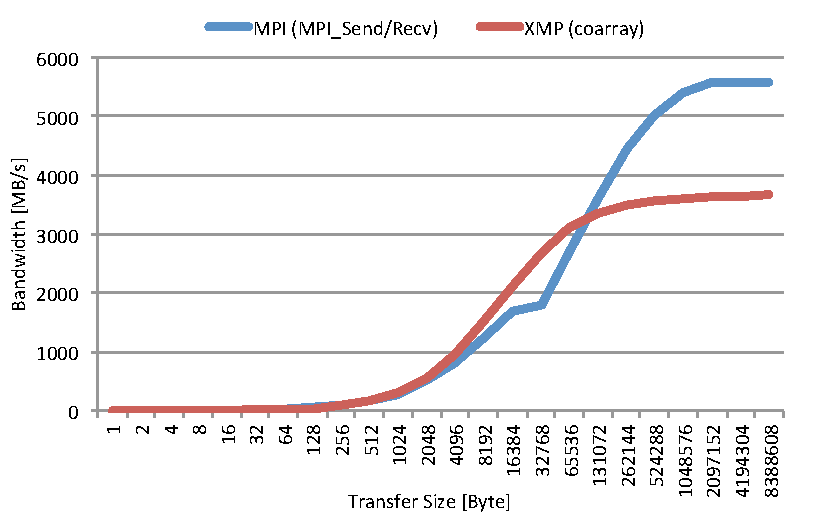
\includegraphics[width=9cm, bb=0 0 390 254]{./figure/comm.pdf}
\caption{Ping-Pong communication bandwidth with MPI (MPI\_Send/Recv) and XMP (coarray).}
\label{comm}
\end{center}
\end{figure}


\begin{table}[t]
\begin{center}
\caption{Evaluation of the weak scaling of decomposition for each domain using problems ranging from 16 to 512 processes.}
{\scriptsize
\label{problem}
\begin{tabular}{l|c|c|c|c} \hline\hline
Problem Size A & Default & Toroidal & Radial & Particle\\ \hline 
mstep & 100 & 20 & 20 & 20 \\
mpsi & 90 & 90 & 90--2880 & 90 \\
mzetamax & 64 & 2--64 & 2 & 2\\
particles per cell & 100 & 100 & 100 & 100--3200\\ \hline
\end{tabular}
}
\end{center}
\end{table}


\begin{table}[t]
\begin{center}
\caption{Process mapping to evaluate the scaling of decomposition for each domain ($N_t$x$N_r$x$N_{rp}$).}
{\scriptsize
\label{decomposition}
\begin{tabular}{l|c|c|c} \hline\hline
Processes & Toroidal & Radial & Particle \\ \hline
16 & $2 \times 2 \times 4$ & $2 \times 4 \times 2$ & $2 \times 2 \times 4$ \\
32 & $4 \times 2 \times 4$ & $2 \times 8 \times 2$ & $2 \times 2 \times 8$ \\
64 & $8 \times 2 \times 4$ & $2 \times 16 \times 2$ & $2 \times 2 \times 16$ \\
128 & $16 \times 2 \times 4$ & $2 \times 32 \times 2$ & $2 \times 2 \times 32$ \\
256 & $32 \times 2 \times 4$ & $2 \times 64 \times 2$ & $2 \times 2 \times 64$ \\ 
512 & $64 \times 2 \times 4$ & $2 \times 128 \times 2$ & $2 \times 2 \times 128$ \\ \hline

\end{tabular}
}
\end{center}
\end{table}



\begin{figure}[t]
\begin{center}
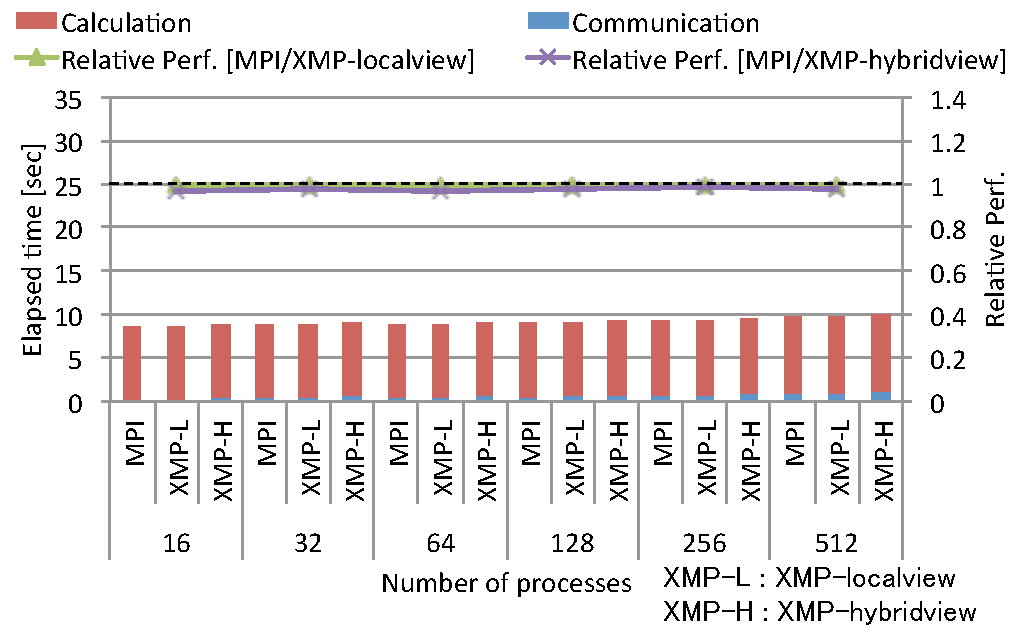
\includegraphics[width=8cm, bb=0 0 492 306]{./figure/toroidal_w.pdf}
\caption{Elapsed time of the decomposition on toroidal dimension from 16 to 512 processes in weak scaling.}
\label{toroidal_w}
\end{center}
\end{figure}


\begin{figure}[t]
\begin{center}
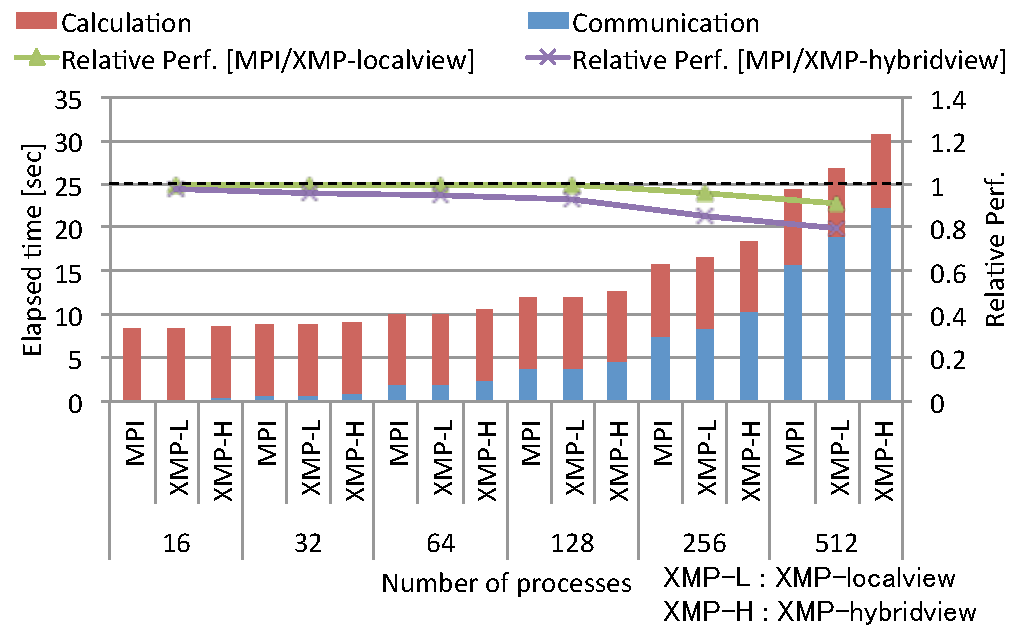
\includegraphics[width=8cm, bb=0 0 492 306]{./figure/radial_w.pdf}
\caption{Elapsed time of the decomposition on radial dimension from 16 to 512 processes in weak scaling.}
\label{radial_w}
\end{center}
\end{figure}


\begin{figure}[t]
\begin{center}
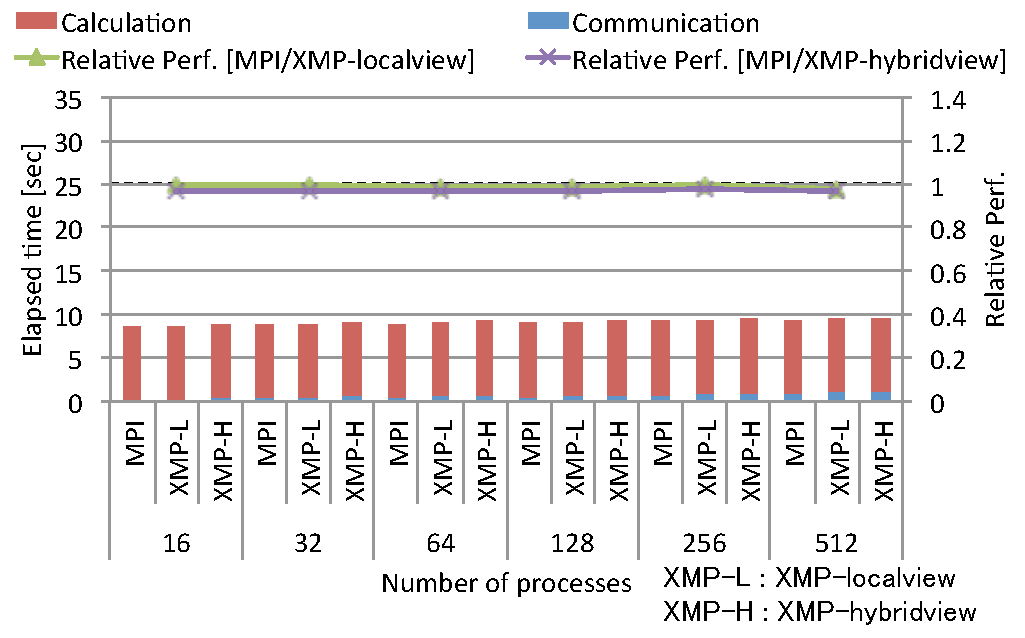
\includegraphics[width=8cm, bb=0 0 492 306]{./figure/particle_w.pdf}
\caption{Elapsed time of the decomposition on particle dimension from 16 to 512 processes in weak scaling.}
\label{particle_w}
\end{center}
\end{figure}



\begin{table}[t]
\begin{center}
\caption{Load imbalance: maximum and minimum times required to calculate the processes with toroidal, radial, and particle decomposition [sec] (number of local grid points in each poloidal plane).}
{\scriptsize
\label{weaktime}
\begin{tabular}{l|c|c} \hline\hline

& \multicolumn{2} {c} {Toroidal} \\ \hline 
Processes & Minimum & Maximum \\ \hline
16 & 8.408406 (19805) & 8.548204 (19916)\\
32 & 8.440145 (19805) & 8.541321 (19916)\\
64 & 8.44846 (19805) & 8.631631 (19916)\\
128& 8.511492 (19805) & 8.718713 (19916)\\
256 & 8.6418 (19805) & 8.853517 (19916)\\
512 & 8.865397 (19805) & 9.109388 (19916)\\ \hline \hline
& \multicolumn{2} {c} {Radial} \\ \hline
Processes & Minimum & Maximum \\ \hline
16 & 8.114932 (10967) & 8.270015 (16164)\\
32 & 8.083982 (12104) & 8.539186 (24200)\\
64 & 8.075058 (14130) & 9.487029 (33462)\\
128 & 8.070919 (17422) & 11.014277 (74745)\\
256 & 8.232447 (23198) & 12.686402 (141700)\\
512 & 8.763279 (34522) & 16.508915  (270844)\\ \hline \hline
& \multicolumn{2} {c} {Particle} \\ \hline
Processes & Minimum & Maximum \\ \hline
16 & 8.408406 (19805) & 8.548204 (19916)\\
32 & 8.406107 (19805) & 8.558563 (19916)\\
64 & 8.394203 (19805) & 8.565195 (19916)\\
128 & 8.394159 (19805) & 8.562974 (19916)\\
256 & 8.393343 (19805) & 8.591214 (19916)\\
512 & 8.390172 (19805) & 8.641762 (19916)\\ \hline
\end{tabular}
}
\end{center}
\end{table}


\begin{figure}[t]
\begin{center}
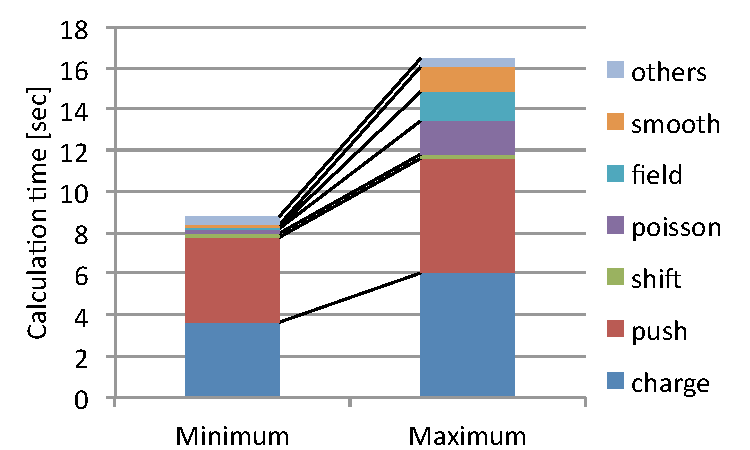
\includegraphics[width=6cm, bb=0 0 360 216]{./figure/loadimbalance.pdf}
\caption{Breakdown of the minimum and maximum calculation times on the radial domain decomposition using 512 processes.}
\label{load}
\end{center}
\end{figure}


\begin{figure}[t]
\begin{center}
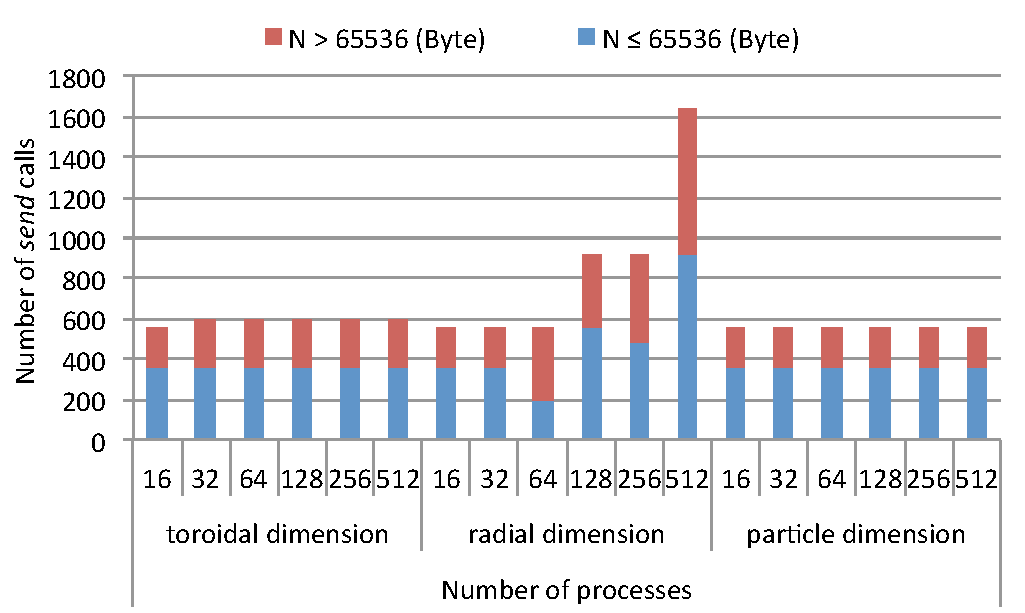
\includegraphics[width=8cm, bb=0 0 492 294]{./figure/comm_w.pdf}
\caption{Number of {\tt send} calls in process number 0 on each domain decomposition from 16 to 512 processes in weak scaling. }
\label{comm_w}
\end{center}
\end{figure}







\begin{figure}[t]
\begin{center}
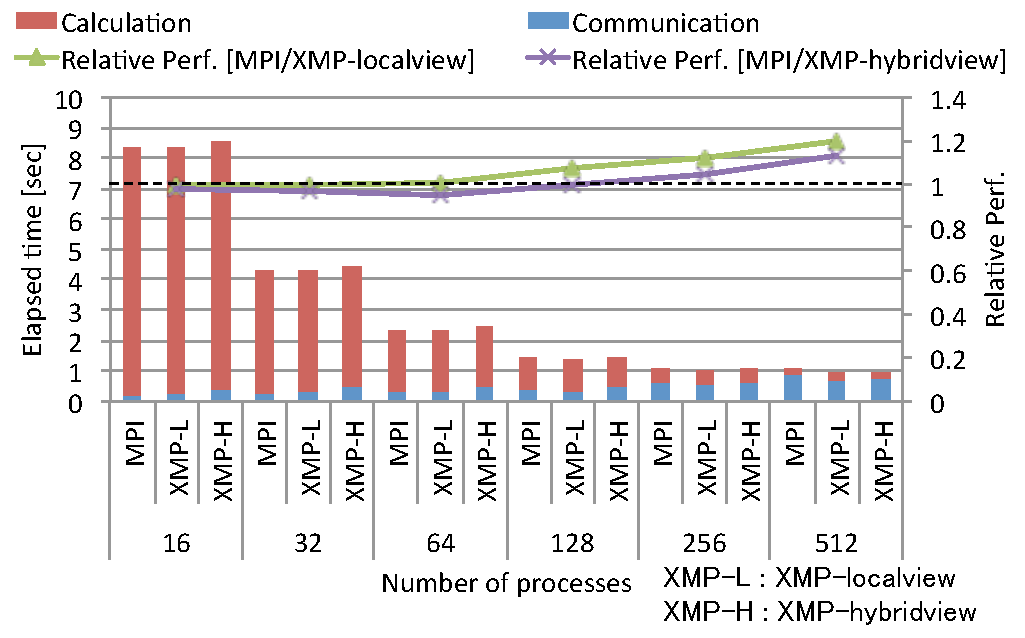
\includegraphics[width=8cm, bb=0 0 492 306]{./figure/radial_s.pdf}
\caption{Elapsed time of the decomposition on radial dimension from 16 to 512 processes in strong scaling.}
\label{radial_s}
\end{center}
\end{figure}


\begin{figure}[ht]
\begin{center}
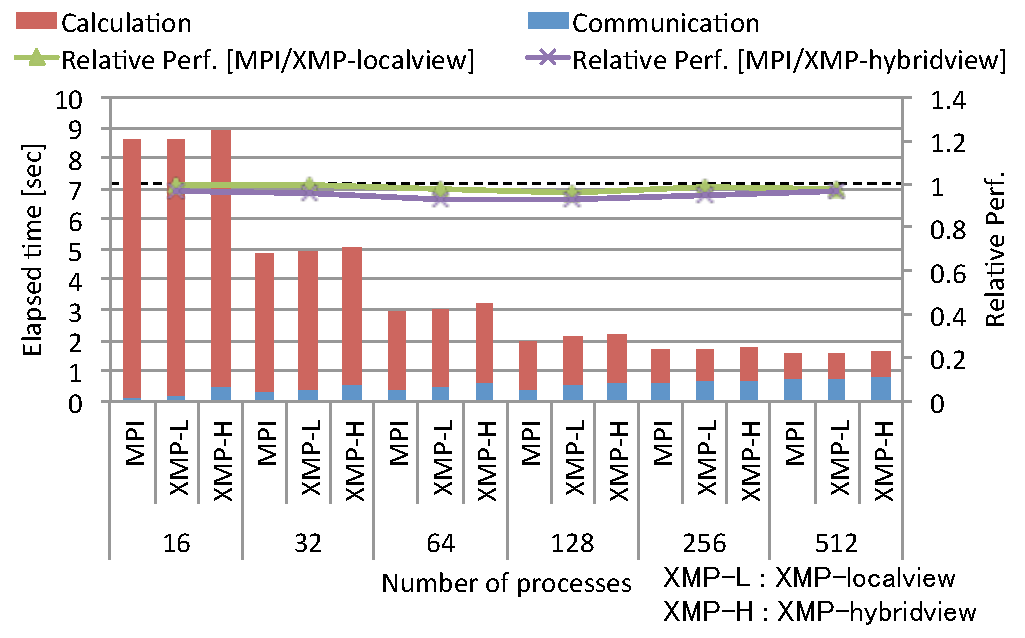
\includegraphics[width=8cm, bb=0 0 492 306]{./figure/particle_s.pdf}

\caption{Elapsed time of the decomposition on particle dimension from 16 to 512 processes in strong scaling.}
\label{particle_s}
\end{center}
\end{figure}


\begin{figure}[t]
\begin{center}
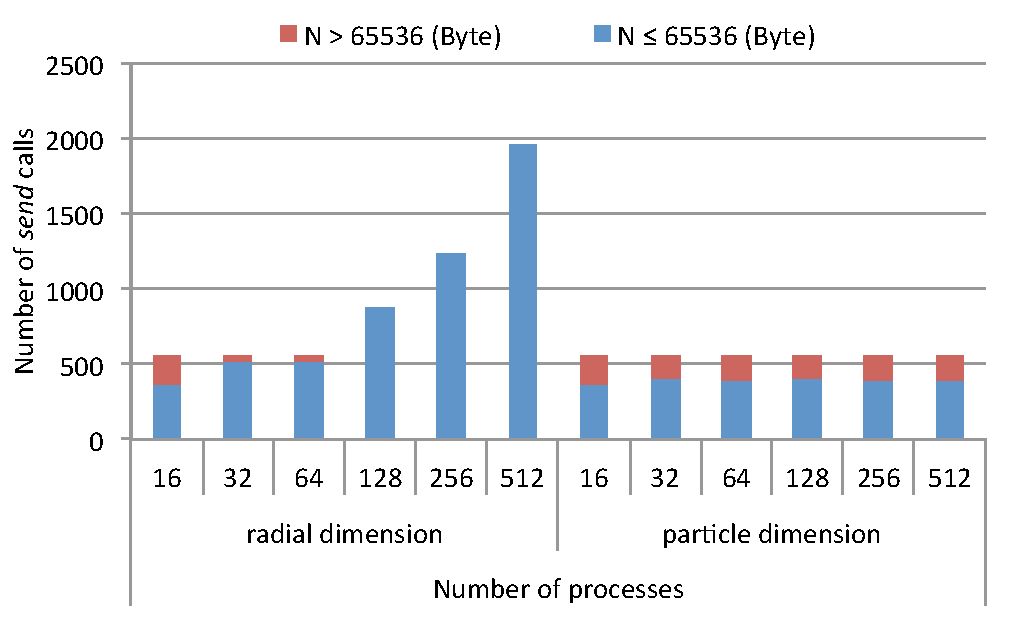
\includegraphics[width=8cm, bb=0 0 492 294]{./figure/comm_s.pdf}
\caption{Number of {\tt send} calls in process number 0 on each domain decomposition from 16 to 512 processes in strong scaling.}
\label{comm_s}
\end{center}
\end{figure}







\begin{figure}[t]
\begin{center}
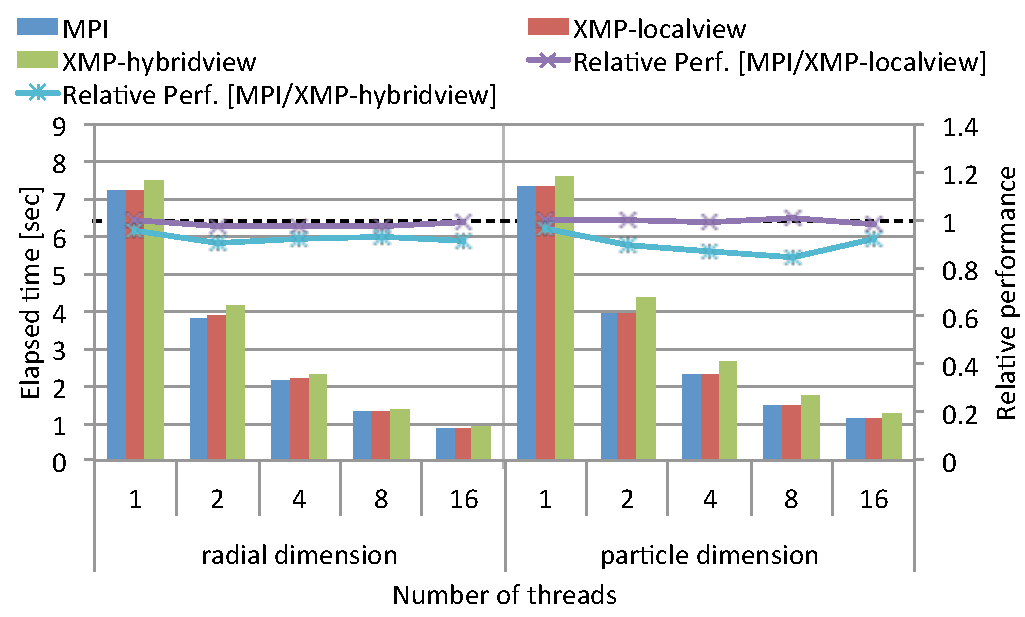
\includegraphics[width=8cm, bb=0 0 492 294]{./figure/omp.pdf}
\caption{Elapsed time of the decomposition on radial and particle dimension from 1 to 16 threads.}
\label{mop}
\end{center}
\end{figure}


%6
\section{Performance Evaluation\label{sec4}}

%6.1
\subsection{Experimental Setting}
We evaluated the performance of our two implementations using a massively parallel GPU cluster: HA-PACS\cite{HAPACS} at the Center for Computational Sciences, University of Tsukuba. Table \ref{env} shows the computing environment employed for one node. HA-PACS is a GPU cluster, but we only utilized CPUs in this study, although we aim to extend our implementation with GPU acceleration in the near future, which is why we decided to use this machine as our platform. We apply the optimization option for NUMA with {\tt 'numactl --localalloc'}, and disable the CPU affinity setting of MVAPICH2 with {\tt MV2\_ENABLE\_AFFINITY=0}.

As preliminary evaluations, we investigate the amount of the memory usage and the performance of communication using XMP and MPI. First, we indicate the comparison of the memory usage when one array is allocated in the local-view model, global-view model, and MPI. They are evaluated with {\tt 'getpid()'} and {\tt 'grep VmHWM /proc/[pid]/status'} from C program during execution. An array size is 1MB. We show the minimum size in the each amount of the memory usage when 4 node execution. The tests showed that the amount of memory usage of all programming models is almost same according to Table \ref{mem}. Then, we evaluate the performance of XMP and MPI communication with Ping-Pong program, which is defined by a power of two communication size, because XMP coarray is implemented by GASNet\cite{GASNET} which is a communication library optimized for some interconnections, e.g., Infiniband and Gemini. Figure \ref{comm} shows the performance of XMP coarray and {\tt MPI\_Send/Recv} communication. XMP is a good performance if the transfer size is about 65536 Bytes or less, whereas MPI is a good performance if it is more than about 65536 Bytes. We used a parameter of GASNet {\tt GASNET\_IBV\_PORTS="mlx4\_0:1+mlx4\_0:2"} which shows to use two ports of Infiniband, but we could get the performance of only single port of Infiniband. It may be an issue with GASNet library.

The GTC-P simulation size is determined by several important numerical parameters. Table \ref{problem} shows the default parameters for problem size A provided by GTC-P, where we modified the parameters to evaluate weak scaling based on problem size A. Strong scaling was evaluated using the minimum parameters in the decomposition of each domain shown in Table \ref{problem}, where {\tt mstep} is the number of calculation steps, {\tt mzetamax} is the number of grid points in the toroidal dimension, and {\tt mpsi} is the number of grid points in the radial domain. Because the number of grid points in the poloidal plane and in the toroidal domain must be the same during decomposition, this was also changed in the parameter set for problem size A. 

First, we used up to 32 nodes of HA-PACS where 16 processes ran on each node and the total number of processes ranged from 16 to 512. The processes mapped to evaluate the decomposition on each domain are shown in Table \ref{decomposition}. As described above, three problem dimensions were considered: toroidal, radial, and particle. When we decomposed these dimensions into parallel processes, we always fixed the decomposition number on two dimensions (e.g., toroidal and radial) as 2 $\times$ 2 and we varied the decomposition size in the other dimension (e.g., particle) from 4 to 128, thereby scaling the total number of processes from 16 to 512. However, during decomposition on the toroidal dimension, we fixed the decomposition number on the radial and particle dimensions as 2 $\times$ 4. This was due to variations in the number of calculations because increasing the toroidal dimension also changes the poloidal planes, as described above. We used this scheme to change the scaling dimension. 

Second, we used 16 nodes where one process ran on each node and the number of threads ranged from 1 to 16 in each process.  The processes mapped on each domain to evaluate the decomposition are 2 $\times$ 4 $\times$ 2 and 2 $\times$ 2 $\times$ 4.


%6.2
\subsection{Results}
With weak scaling, Figures \ref{toroidal_w}, \ref{radial_w} and \ref{particle_w} shows the elapsed time for both calculation and communication of MPI, XMP-localview and XMP-hybridview required to scale the number of processes from 16 to 512, where decomposition on the toroidal and particle dimensions exhibited good scalability whereas scaling on the radial dimension was poor. Figure \ref{radial_w} shows that the performance of decomposition on the radial dimension decreased as the number of nodes increased compared with the other two types of domain decomposition, as shown in Figures \ref{toroidal_w} and \ref{particle_w}. Most of the communications are performed at the neighboring surface during decomposition on any dimension and the total amount of communication data does not vary greatly; thus, we focused on the calculation load balance between processes. Table \ref{weaktime} shows the difference between the maximum and minimum calculation times required for each type of decomposition, where the calculation time was defined as the computational time required for each process except the communication time. This table shows that the calculation time for processes differed greatly with radial dimension decomposition as the number of processes increased. This phenomenon occurred with all three implementations, including MPI.

This may be explained by the method used to decompose the domain in the radial dimension. For other dimensions, it is easy to decompose the domain completely and equally for all processes. However, decomposition is complicated in the radial dimension because the domain volume varies in the inner part and outer part due to the torus form of the problem space. The volume and the corresponding grid size are calculated based on the formula used to describe the torus shape, which implies that an error is incurred during integer rounding to determine the number of grids. Table \ref{weaktime} shows that the number of total grid points assigned to the processes with the maximum and minimum calculation times differed greatly. Also, Figure \ref{load} shows the breakdown of the minimum and maximum calculation times on the radial domain decomposition 512 processes. The difference between the calculation times of the grid-related works, such as {\tt charge}, {\tt push}, {\tt poisson}, {\tt field}, and {\tt smooth}, increased on radial domain decomposition. During each time step, the computation of all processes must be bounded as a barrier operation and the increase in the integer rounding error according to the problem size (i.e., weak scaling) causes a greater load imbalance, which degrades the overall performance. 

On the other hand, the communication time of XMP-localview and XMP-hybridview on the radial dimension increases as the number of nodes increased compared with the MPI, as shown in Figure \ref{radial_w}. We explored the number of {\tt send} calls and each communication size because the performance of communication on XMP and MPI are reversed at about 65536 Bytes according to Figure \ref{comm}. Figure \ref{comm_w} shows the number of {\tt send} calls in process number 0 on each domain decomposition classified as the communication size of more than 65536 Bytes and 65536 Bytes or less. In the radial domain decomposition, the number of {\tt send} calls at more than 65536 Bytes increases compared with the toroidal and particle decomposition. Therefore, the performance of XMP-localview and XMP-hybridview is degraded compared with MPI. The results were the XMP-localview implementation obtains approximately the same performance as the MPI implementation while the performance degradation using XMP-hybridview is increased by up to 20\% compared with the MPI implementation. Currently, we are under investigation why the number of {\tt send} calls increased on the radial domain decomposition in weak scaling.

With strong scaling, Figures \ref{radial_s} and \ref{particle_s} show the elapsed time for both calculation and communication of MPI, XMP-localview and XMP-hybridview, where the decomposition on the radial and particle dimensions, respectively. The performances of XMP-localview, and XMP-hybridview on the particle dimension are almost same compared with MPI, as shown Figure \ref{particle_s}, while the elapsed time of the decomposition on the radial dimension increases as the number of nodes increased, as shown Figure \ref{radial_s}. 

We explored the number of {\tt send} calls and each communication size same as weak scaling. Figure \ref{comm_s} shows the number of {\tt send} calls in process number 0 on radial and particle domain decomposition classified as the communication size of more than 65536 Bytes and 65536 Bytes or less. The number of {\tt send} calls on the radial domain decomposition at 65536 Bytes or less increases compared with the particle decomposition. Therefore, the performance of XMP-localview and XMP-hybridview are increased compared with MPI on radial domain decomposition from 128 to 512 processes in strong scaling.

Figure \ref{mop} shows the elapsed time of the decomposition on radial and particle dimension, i.e., 2 $\times$ 4 $\times$ 2 and 2 $\times$ 2 $\times$ 4, ranged from 1 to 16 threads per process using 16 nodes where one process ran on each node. The results were the performance of XMP implementation with thread parallelization is scaled the same as MPI.


\begin{table}[t]
\begin{center}
\caption{Differences in the delta SLOC from Serial implementation for several different implementations of GTC-P.}
{\scriptsize
\label{gtcp_code}
\begin{tabular}{c|c|c|c|c} \hline\hline
 & \multirow{2}{*}{Serial} & \multirow{2}{*}{MPI} & \multicolumn{2}{c}{XMP} \\ \cline{4-5}
 & & & localview & hybridview \\ \hline
SLOC			& 4110 	& 5427 	& 5398 	& 5179\\ \hline
modified 			& - 		& 170 	& 168 	& 158\\ 
added     			& -    	& 1319 	& 1303 	& 1112\\
deleted   			& - 		& 2 		& 15 		& 43\\ \hline
Total delta SLOC 	& - 		& 1491	& 1486 	& 1313\\ \hline
\end{tabular}
}
\end{center}
\end{table}


\begin{figure}[t]
\begin{center}
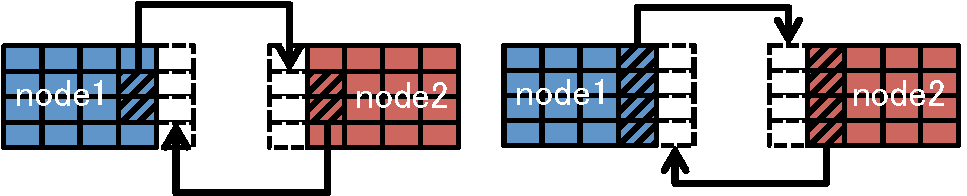
\includegraphics[width=8cm, bb=0 0 464 94]{./figure/sleeve.pdf}
\caption{Updating of the sleeve area with MPI and XMP-localview (left), and XMP-hybridview (right) in GTC-P. The hatching areas are communicated to nearby node.}
\label{sleeve}
\end{center}
\end{figure}


%6.3
\subsection{Productivity and Performance}
A good programming environment should facilitate high performance and high productivity, but high performance is sometimes obtained by low-level programming such as MPI, which unfortunately yields low productivity. 

The XMP-localview implementation is simple and intuitive compared with MPI because the coarray communication is expressed in the form of an array assignment statement, as shown Figures \ref{pmove_xmp} and \ref{coarray}. In coarray notation, the communication size and data are intuitively represented by array section and the data type is checked automatically. The performance of XMP-localview is comparable to that of the MPI version. 

In XMP-hybriview, the global data structure required for the field data is described in the global-view model, which is almost the same as that in the serial code without particle calculation to communicate to the other process, and its data distribution is annotated by the directives, as shown in Figure \ref{gblock}. This improves the readability of the code because it is unnecessary for users to describe the many arguments on a line such as MPI APIs, thereby facilitating the easy maintenance of the program and simple parallelization from the original sequential code. For the global data structure, the communication with the overlapped sleeve area in the distributed calculation domain can be described in only one line of the {\tt reflect} directive, as shown in Figure \ref{reflect}.

Table \ref{gtcp_code} shows the delta Source Lines Of Code (SLOC) \cite{SLOC} for several implementations. This metric indicates how many lines of code changed from the serial implementation of GTC-P, which shows modified, added, and deleted lines. Due to the reasons described above, the amount of code added and modified from the serial implementation is smaller with the XMP-hybridview implementation than the MPI implementation. In both of XMP implementations, the deleted lines are larger than MPI implementation because the explicit memory free is unnecessary for the distributed array and communication buffer for coarray in the global scope. In summary, XMP-hybridview implementation increases productivity.

The difference in performance between XMP-hybridview and MPI is attributable to the increase in the communication size of the {\tt reflect} directive. The {\tt reflect} directive is responsible for the communication designated as the sleeve area by the {\tt width} clause, but it cannot update partially sleeve area. Figure \ref{sleeve} shows that the two-dimensional array is distributed to two nodes and exchanged the sleeve area in MPI and XMP implementations. In GTC-P, there is the communication pattern updated only inner sleeve area which is represented as the hatching areas in Figure \ref{sleeve} (left).


\section{Related Research \label{sec5}}

GTC or GTC-P have been executed and optimized on some platforms. X. Liao et al.\cite{PHI-GTC} optimized GTC to use offload-programming model for the Intel Xeon Phi accelerator, and evaluated the performance on MilkyWay-2 supercomputer. K. Madduri et al.\cite{MANY-GTC} described the optimization for multi- and many-core systems, and evaluated on some systems including Graphic Processing Unit (GPU) based on NVIDIA Fermi architectures. In our study, we focus on the evaluation of not only the performance but also the productivity for GTC-P.

PIC method is often implemented some PGAS parallel programming languages. H. Sakagami and T. Mizuno\cite{HPF-PIC} implemented 2D particle code, ESPAC2: 2D electro-static plasma, based on PIC method using High Performance Fortran (HPF) \cite{HPF} which is directive-based language similar to OpenMP and supports the global-view model. The particle data is distributed into the block, while the electrostatic field is replicated onto each process. After the distributed particle data is calculated in each process, the reduction operation is executed to update the particle data of electrostatic field on each time step. The data distribution is an easy expression which is annotated by directives in HPF.  R. Preissl et al.\cite{CAF-GTC} introduced hybrid PGAS+OpenMP approach for 3D PIC code, Gyrokinetic Tokamak Simulation (GTS) which is implemented in MPI+OpenMP. As PGAS parallel programming language, they used Coarray Fortran. The one-sided communication in Coarray Fortran is simple and more intuitive notation compared with MPI programming because it is expressed in the form of array assignment statement. However, the description of data distribution is same as MPI. To use simple coarray communication and easy data distribution by directives, we consider a hybrid-view approach, which combines the global-view and local-view models in XMP. 

%7
\section{Conclusion\label{sec6}}
In this study, we implemented two versions of GTC-P, a large-scale nuclear fusion simulation code, using the global-view and local-view programming models in XMP for parallel programming languages, and we evaluated their performance and productivity. The first version, XMP-localview, only uses coarray communication in the local-view programming model, which simply replaces MPI point-to-point communication, except for collective communication such as MPI\_Allreduce. The second version, XMP-hybridview, uses the distribution of the calculation domain and the {\tt reflect} directive in the global-view programming model, as well as coarray communication for particle motion in the local-view programming model. Experimental evaluations showed that the XMP-localview implementation obtained approximately the same performance as MPI, whereas the XMP-hybridview implementation degraded the performance by 20\%. In addition, we obtained high productivity with the XMP implementation. In XMP-localview, the coarray notation is simpler and more intuitive compared with MPI programming, and the XMP-hybridview allows more natural data expression for both static grid space data (in the global-view model) and dynamic particle data (in the local-view model), thereby increasing the readability of the code.


